\documentclass[informe.tex]{subfiles}
\begin{document}

En este tipo de filtro el parámetro característico es que el orden es dependiente de las atenuaciones elegida para cada banda.\newline

\textbf{Función de aproximación}\newline
La función de aproximación queda dada por 
	
				\[ B_n(\omega)=\omega^n \]
	
\textbf{Respuesta en frecuencia}\newline
	
				\[ \left| H(j\omega) \right|^2 = \frac{1}{1+ \omega^{2n}} \]
	
	\begin{tabular}{p{0.45\textwidth} p{0.5\textwidth}}		
		
			
		\begin{wrapfigure}{l}{0.9\linewidth}
		\centering
		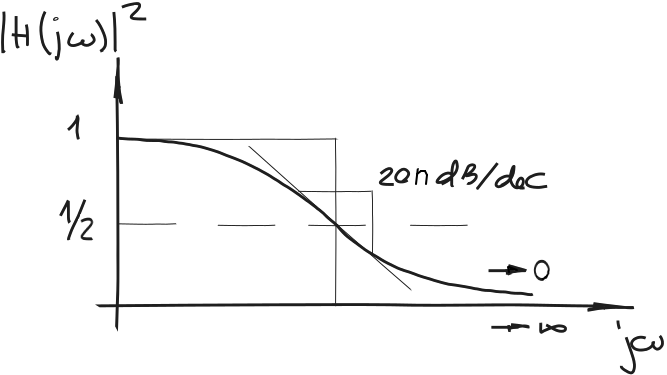
\includegraphics[width=\linewidth]{butterworth_1.png}
		\caption{Respuesta en frecuencia del filtro de Butterworth}
		\end{wrapfigure}				
		&
		Resumen de propiedades: 
		\newline
		1- Valores característicos:
		{
			$ \left| H(j0) \right|^2 = 1 ,
			\left| H(j1) \right|^2 = \frac{1}{2} ,(3dB),
			\left| H(j\infty) \right|^2 = 0 
			$
		}\newline\newline
		2- Monótona decreciente  para $\omega \geq 0 $.\newline 
		
		3- Magnitud máxima plana, significa que la derivada $(2n-1)$-ésima es cero en $\omega=0$.\newline 
		
		4- La pendiente de decaimiento (roll of) es de $20n $dB/dec para orden $n$.
		\\ 
	\end{tabular} \newline\newline\newline\newline\newline
		
		
\textbf{Orden del filtro y atenuación}\newline
			
En base a las características enunciadas anteriormente se llega a que el orden queda dado en función de la atenuación requerida según la banda de interés:
					\[
						n= \frac{log_{10}(10^{A_{db}/10} - 1)}
						       {2log_{10} \omega}
					\]\newline
\underline{Desarrollo}\newline
					 \[
						\left | H(j \omega ) \right |^2_{db}
						=
						10 log_{10} \frac{1}{1+\omega^{2 n}} = -A_{dB}
					\]
					 \[
						\omega^{2n} = 10^{A_{dB}/10} - 1					
					\]
					 \[
						2n log_{10} \omega = log_{10}( 10^{A_{db}/10}-1) \longrightarrow n= \frac{log_{10}(10^{A_{db}/10} - 1)}
						       {2log_{10} \omega}
					\]\newline
											 
\textbf{Función de transferencia y polos de la función de transferencia}\newline	 	
			  
	La función de transferencia tiene la forma:

        $$
		\left| H(s)) \right|^2 =
		\left \{ 
		    \begin{matrix}
		    \frac{1}{1 + s^{2n}} & \mbox{, si n es par}  \\
       		\frac{1}{1 - s^{2n}} & \mbox{, si n es impar}
		    \end{matrix}
		\right.		
		$$	
		$$
			H(s)=
				\prod_{k=1}^{n}{\frac{1}{s - s_k}}
				=
				\left \{ 
			    \begin{matrix}
			       \prod_{k=1}^{n/2} {\frac{1}{s^2 + 2 sin \theta_k + 1}}
                           & 
                                 \mbox{, si n es par}  \\
		       \frac{1}{s+1} \prod_{k=1}^{n/2} {\frac{1}{s^2 + 2 sin \theta_k + 1} }
                           & 
                                   \mbox{, si n es impar}  
	    \end{matrix}
\right.		
        $$
La expresión para determinar los polos queda dada por 
	$$
		\hat{s}_k = - sin \left( \frac{2k-1}{2n} \right) \pi + j  cos \left( \frac{2k-1}{2n} \pi \right)
	$$        
donde $k$ y $n$ es es un número entero dado entre $k=1$,$2$,...,$n$.
		
\underline{Desarrollo}\newline

   Para el caso de que $n$ sea par se tiene:\newline
	\begin{center}
		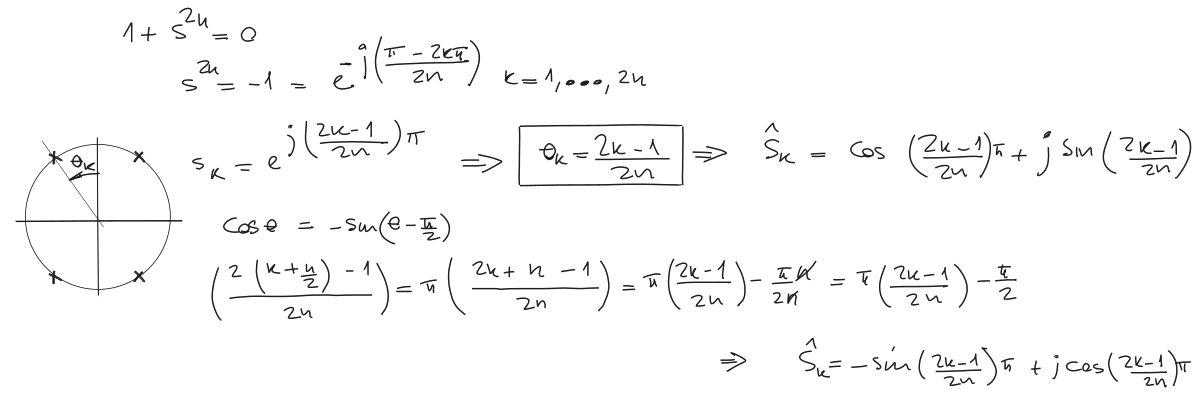
\includegraphics[scale=0.37]{butterworth_2.png}
	\end{center}

 	Y en el otro caso, donde $n$ es impar el desarrollo consiste en:\newline
 	
	\begin{center}
		\centering 
		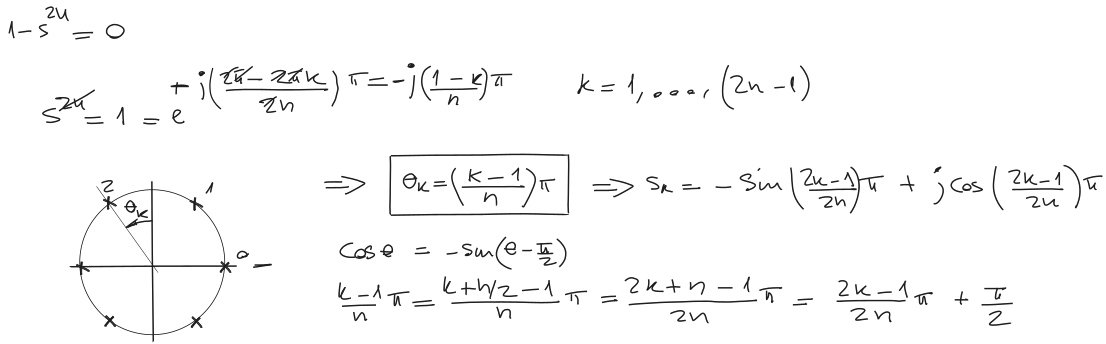
\includegraphics[scale=0.37]{butterworth_3.png}
	\end{center}
    		    		
    Finalmente, construyendo las expresiones correspondientes con cada polo y su conjugado tendrá la siguiente forma:\newline		
    \begin{center} 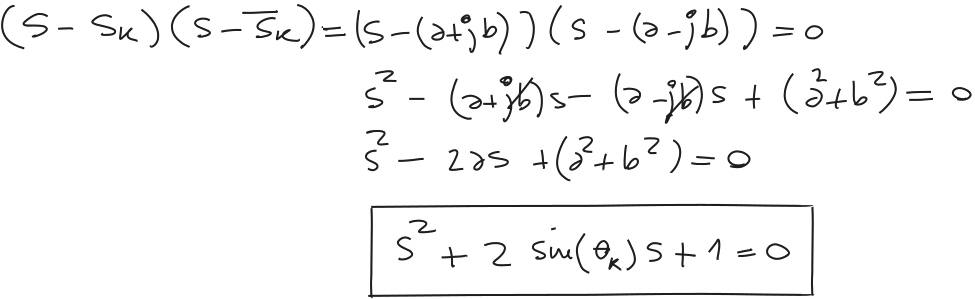
\includegraphics[scale=0.3]{butterworth_4.png}	\end{center}

%%
    		
\textbf{Ejemplo 1 con Matlab:} Determinando los polos y los ceros para orden 3, Fig. \ref{fig:func:butterworth:ej1}.\newline 
   
En este ejemplo se construye la función de transferencia a partir de los polos conjudados.\newline

\lstinputlisting[language=Matlab, frame=single]{./src_matlab/butterworth_ej1.m}
		 	
%%  
\textbf{Ejemplo 2 con Matlab:} Determinando polos y ceros para orden 3, Fig. \ref{fig:func:butterworth:ej1}.\newline  
  
A diferencia del ejemplo anterior, se determina la función de transferencia calculando los polos individuales en el semiplano-izquierdo y luego se hace el producto de cada expresión correspondiente.\newline 

\lstinputlisting[language=Matlab, frame=single]{./src_matlab/butterworth_ej2.m}   		
    
\begin{figure}
		\centering
		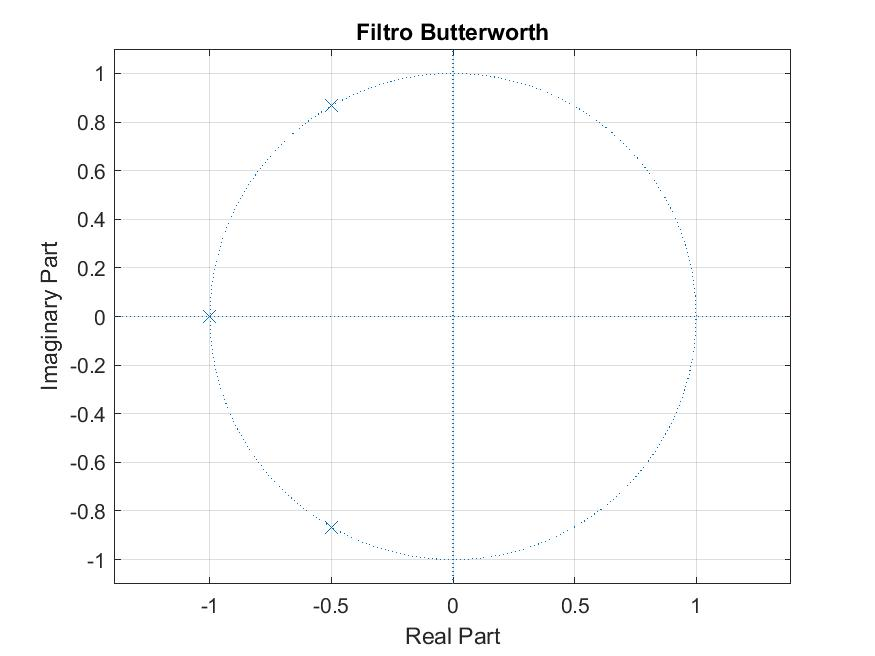
\includegraphics[scale=0.4]{butterworth_pz_ej1.jpg}
		\caption{Diagrama de polos y ceros de la función de transferencia, $H(s)$, del filtro de Butterworth}
		\label{fig:func:butterworth:ej1}
\end{figure}   
    		
\end{document}
